\documentclass{article}
\usepackage{tikz}
\usepackage{amsmath}
\usepackage{wrapfig}
\usetikzlibrary{arrows.meta,positioning,decorations.pathreplacing}

% if you need to pass options to natbib, use, e.g.:
\PassOptionsToPackage{numbers, compress}{natbib}
% before loading neurips_2024


% ready for submission
\usepackage[preprint]{neurips_2024}


% to compile a preprint version, e.g., for submission to arXiv, add add the
% [preprint] option:
%     \usepackage[preprint]{neurips_2024}


% to compile a camera-ready version, add the [final] option, e.g.:
    % \usepackage[final]{neurips_2024}


% to avoid loading the natbib package, add option nonatbib:
%    \usepackage[nonatbib]{neurips_2024}


\usepackage[utf8]{inputenc} % allow utf-8 input
\usepackage[T1]{fontenc}    % use 8-bit T1 fonts
\usepackage{hyperref}       % hyperlinks
\usepackage{url}            % simple URL typesetting
\usepackage{booktabs}       % professional-quality tables
\usepackage{amsfonts}       % blackboard math symbols
\usepackage{nicefrac}       % compact symbols for 1/2, etc.
\usepackage{microtype}      % microtypography
\usepackage{xcolor}         % colors


\title{CSE 250A Final Project\\Predicting Coding and Noncoding Sequences in Eukaryotic DNA}

% The \author macro works with any number of authors. There are two commands
% used to separate the names and addresses of multiple authors: \And and \AND.
%
% Using \And between authors leaves it to LaTeX to determine where to break the
% lines. Using \AND forces a line break at that point. So, if LaTeX puts 3 of 4
% authors names on the first line, and the last on the second line, try using
% \AND instead of \And before the third author name.


\author{
    Tej Gaonkar \\
    \texttt{tgaonkar@ucsd.edu} \\
    \And
    Conor Mc Gartoll \\
    \texttt{cmcgartoll@ucsd.edu} \\
    \And
    Justin Vincent Shen \\
    \texttt{jvshen@ucsd.edu}\\
    \And
    Jared Ziv\\
    \texttt{j1ziv@ucsd.edu} \\
  % examples of more authors
  % \AND
  % Coauthor \\
  % Affiliation \\
  % Address \\
  % \texttt{email} \\
  % \And
  % Coauthor \\
  % Affiliation \\
  % Address \\
  % \texttt{email} \\
  % \And
  % Coauthor \\
  % Affiliation \\
  % Address \\
  % \texttt{email} \\
}


\begin{document}


\maketitle


\section{Problem Description}

A fundamental task in computational biology is to identify functional regions within genomic DNA, specifically predicting the probability of $k$ sequential nucleotides (k-mer) being part of a coding or noncoding region. Coding sequences (CDS) define the small percentage of DNA (approximately 1\% in humans\cite{zhao_encode_deciphering_2025}) that are converted into mRNA, and finally into amino acid sequences as proteins. Noncoding sequences (NCS), alternatively, make up about 99\% of our genome and are essential in the control of gene activity, including sequences such as introns, promoters, enhancers, etc.

The accurate classification of these regions is important for many tasks in biological fields, such as comparative genomics, genome annotations, gene predictions, etc. Due to the prevalence of genomic DNA data sets, probablistic modeling is a great solution to learn to distinguish between CDS and NCS. Specifically we found this to be a great application for a Hidden Markov Model (HMM).

\section{Data Sourcing and Processing}

\subsection{Sourcing}
Our dataset comes from the National Center of Biotechnology Information (NCBI)'s RefSeq. RefSeq provides entire annotated genomes in the form of a FASTA file and a GFF file.

More specifically, we used the \textit{Saccharomyces cerevisiae} genome\cite{scerevisiae_s288c_r64}. It served as an ideal genome for initial model development, because it is both well annotated and reasonable in size. We avoided the use of a larger genome, largely because the time complexity of the forward, backward, and Viterbi algorithms would make training incredibly time consuming on a massive dataset.

\subsection{Processing}
Our data was processed using the \verb|gffutils| and \verb|biopython| libraries. The NCBI page provides the \verb|.fasta| file, which encodes the entire genome, and the \verb|.gff| file, which provides annotation on DNA structures.

To create the training data, we labeled each 3-mer in the genome as coding or noncoding. A 3-mer was considered coding if the central nucleotide was present within a sequence with feature "CDS" in the \verb|.gff| file. Then, each 3-mer was written to a \verb|.csv| file which was used to train the model. We felt that a 3-mer served as a better observation than single nucleotides, because codons can signal the start and end for transcription sites. We check every k-mer, however, because it's not guaranteed that a NCS between two CDS would have a number of nucleotides which is divisible by 3 (i.e. checking \textit{only} each subsequent block of 3 nucleotides may miss a start codon, like a frameshift)

% \paragraph{Draft Note:} In the coming weeks we will try different k-mer sizes, as well as potentially labeling coding data differently or adding more states (e.g. instead of "coding" and "noncoding", perhaps "intron", "exon", "promoter", "UTR", etc.). For now, as a first draft, we felt that this was sufficient to gather feedback and develop upon.

\section{Modeling and Inference}
\subsection{Model Structure}
\begin{wrapfigure}{r}{0.45\textwidth}
\centering
\vspace{-10pt}
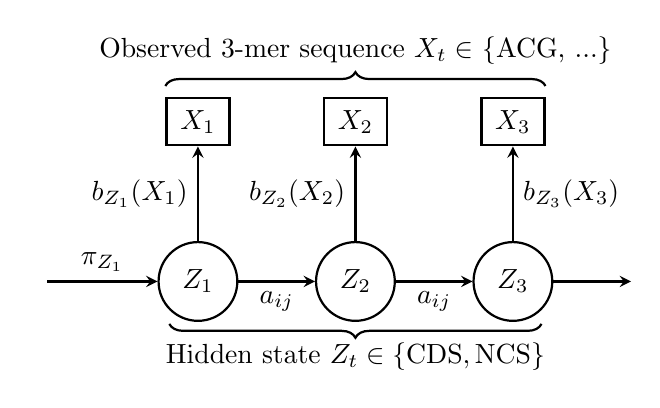
\begin{tikzpicture}[
    node distance=2cm,
    >=stealth,
    thick,
    state/.style={circle,draw,minimum size=10mm},
    obs/.style={rectangle,draw,minimum width=8mm,minimum height=6mm}
]

% Hidden states
\node[state] (z1) {$Z_1$};
\node[state,right of=z1] (z2) {$Z_2$};
\node[state,right of=z2] (z3) {$Z_3$};

% Observations
\node[obs,above=1.2cm of z1] (x1) {$X_1$};
\node[obs,above=1.2cm of z2] (x2) {$X_2$};
\node[obs,above=1.2cm of z3] (x3) {$X_3$};

% Transitions between hidden states
\draw[->] (z1) -- (z2) node[midway,below] {$a_{ij}$};
\draw[->] (z2) -- (z3) node[midway,below] {$a_{ij}$};
\draw[->] (z3) -- ++(1.5,0);

% Emissions
\draw[->] (z1) -- (x1) node[midway,left] {$b_{Z_1}(X_1)$};
\draw[->] (z2) -- (x2) node[midway,left] {$b_{Z_2}(X_2)$};
\draw[->] (z3) -- (x3) node[midway,right] {$b_{Z_3}(X_3)$};

% Initial distribution
\node[left=1.4cm of z1] (start) {};
\draw[->] (start) -- (z1) node[midway,above] {$\pi_{Z_1}$};

% Braces / annotations
\draw [decorate,decoration={brace,amplitude=5pt,raise=5pt,mirror}]
  (z1.south west) -- (z3.south east)
  node[midway,below=8pt] {Hidden state $Z_t \in \{\text{CDS}, \text{NCS}\}$};

\draw [decorate,decoration={brace,amplitude=5pt,raise=4pt}]
  (x1.north west) -- (x3.north east)
  node[midway,above=8pt] {Observed 3-mer sequence $X_t \in $ \{ACG, ...\}};

\end{tikzpicture}
\vspace{-10pt}
\end{wrapfigure}
We develop a Hidden Markov Model (HMM) that accurately classifies a DNA sequence as a CDS or NCS. We apply an HMM because it reflects DNA structure well, since the model takes in a sequence of 3-mer nucleotide observations ($X_t$ such as ACG, TGA, etc.) which have unique functions, reflected by the hidden states ($Z_t$). Each observation is pulled from a genome of length $L$, so that observation sequence length is $T=L-2$ (ignoring incomplete trailing nucleotides), and we iterate through the observations with each 3-mer per timestep. We follow the following conditional independence structure:
\[
P(Z_1) = \pi_{Z_1}, \qquad
P(Z_t \mid Z_{1:t-1}) = P(Z_t \mid Z_{t-1}) = a_{Z_{t-1},Z_t},
\]
\[
P(X_t \mid Z_{1:t}, X_{1:t-1}) = P(X_t \mid Z_t) = b_{Z_t}(X_t),
\]
As shown above, the hidden state is initialized from a distribution, $\pi$. The transition and emission matrices are derived from the conditional independence relationship and are parametrized as $a_{Z_{t-1},Z_t}$ and $b_{Z_t}(X_t)$.

\subsection{Inference/Learning Algorithm}
Since our dataset is fully labeled with the true CDS/NCS state for each 3-mer,
we train the HMM in a supervised manner. We use the
\texttt{hmmlearn} library to initialize a model, specifically \texttt{CategoricalHMM}, which is suited well for binary prediction tasks such as this one. We manually calculate the
initial distribution $\pi$, the transition matrix $A$, and the emission matrix
$B$ from empirical counts in the training set by computing the fraction of training samples that reflect some state, transition, or emission, respectively, and normalizing over the total number of observations in the training set.

During evaluation on the test genome sequence, the true labels are hidden and
must be inferred. We apply the Viterbi algorithm to compute the most probable
sequence of hidden states $Z_{1:T}$ given the observed 3-mer sequence
$X_{1:T}$. This allows us to compare the predicted CDS/NCS hidden state
against the ground-truth genome annotation and measure model accuracy.

\subsection{Simplifications and Assumptions}
Note that as a simplification, we assume each 3-mer is independent and identically distributed. This assumption is necessary, as it allows us to apply the Viterbi algorithm by enabling conditional independence which is essential to the filling of the $\ell^*$ matrix. Without it, the calculation of columns past $t=1$
\begin{align*}
    \ell^*_{j,t+1} = P(s_1,...,s_t,S_{t+1}=j,o_1,...,o_{t+1})
\end{align*}
would not be easily simplified, and as such the calculation would be substantially more difficult, if possible.

\section{Results and Discussion}

We trained our HMM on the \textit{Saccharomyces cerevisiae} 3-mer dataset described in Section~2.1. Each observation $X_t$ is one of the 64 possible nucleotide 3-mers, and the hidden state $Z_t \in \{\text{NCS}, \text{CDS}\}$ indicates whether the central base of the 3-mer lies in a noncoding or coding region. In our implementation, state index 0 corresponds to NCS and index 1 corresponds to CDS.

Using the \texttt{hmmlearn} library, we instantiated a two-state \texttt{CategoricalHMM} with 64 discrete emission categories. The model was trained on an 80\% contiguous split and evaluated on the remaining 20\%. The HMM achieves a test accuracy of \textbf{79.74\%}, substantially above simple baselines.

\subsection*{Baseline Comparisons}

\begin{table}[h]
\centering
\begin{tabular}{lcc}
\toprule
Model & Train Accuracy & Test Accuracy \\
\midrule
Always NCS (majority class) & 0.724 & 0.703 \\
3-mer majority vote         & 0.724 & 0.703 \\
HMM (ours)                  & 0.791 & 0.797 \\
\bottomrule
\end{tabular}
\caption{Accuracy of the HMM compared to simple baselines.}
\end{table}

The 3-mer majority classifier already exploits label frequencies but still plateaus near 70\% accuracy.
Our HMM improves this by nearly 10 percentage points, demonstrating the value of temporal structure.

\subsection*{Learned Transition Structure}

The learned transition matrix is:

\begin{table}[h]
\centering
\begin{tabular}{lcc}
\toprule
 & \multicolumn{2}{c}{$P(Z_{t+1} \mid Z_t)$} \\
\cmidrule(lr){2-3}
Current $Z_t$ & Next = NCS & Next = CDS \\
\midrule
NCS  & 0.998145 & 0.001855 \\
CDS  & 0.000706 & 0.999294 \\
\bottomrule
\end{tabular}
\caption{Learned transition probabilities.}
\label{tab:transition}
\end{table}

Both states show extremely high self-transition probabilities, implying long contiguous coding and noncoding regions. The expected run lengths, computed as $1/(1-P(\text{stay}))$, are approximately 1417 3-mers for NCS and 539 3-mers for CDS, consistent with known genome structure.

\subsection*{Emission Analysis}

Table~\ref{tab:emissions-corrected} lists the top 10 3-mers ranked by absolute difference
$\Delta = P(X\mid \text{CDS}) - P(X\mid \text{NCS})$.

\begin{table}[h]
\centering
\begin{tabular}{lccc}
\toprule
3-mer & $P(X\mid \text{NCS})$ & $P(X\mid \text{CDS})$ & $\Delta$ \\
\midrule
AAA & 0.05046 & 0.03482 & $-0.01563$ \\
TTT & 0.05026 & 0.03477 & $-0.01549$ \\
ATA & 0.03412 & 0.02048 & $-0.01363$ \\
TAT & 0.03396 & 0.02045 & $-0.01351$ \\
TAA & 0.02786 & 0.01964 & $-0.00823$ \\
TTA & 0.02779 & 0.01966 & $-0.00813$ \\
CCA & 0.01027 & 0.01688 & $+0.00661$ \\
TGG & 0.01024 & 0.01669 & $+0.00645$ \\
CAA & 0.01984 & 0.02451 & $+0.00468$ \\
TTG & 0.01984 & 0.02439 & $+0.00455$ \\
\bottomrule
\end{tabular}
\caption{Top 3-mers by absolute emission difference between CDS and NCS, with $\Delta = P(X\mid\text{CDS}) - P(X\mid\text{NCS})$.}
\label{tab:emissions-corrected}
\end{table}

% Add additional analysis of these specific codons and if they are meaningful (stop codon, etc.)

Several interpretable patterns emerge:

\begin{itemize}
    \item The most CDS-enriched 3-mers tend to exhibit more balanced GC content (e.g., CCA, TGG), which aligns with the known pattern of CDS regions containing higher GC content.

    \item Start and stop codon triplets (TAA, TAG, TGA) do not reliably indicate coding regions in this model because 3-mers are extracted overlapping. These motifs frequently appear out of frame inside CDS and also within AT-rich NCS regions, leading the HMM to associate them more with background sequence composition than with true translational boundaries.

    \item The magnitude of enrichment is larger for NCS-specific 3-mers than for CDS-specific ones. This arises because yeast NCS regions are strongly AT-rich and constitute the majority of the genome, producing larger deviations in their 3-mer distribution, whereas CDS regions are constrained by codon usage and therefore exhibit more moderate variation.
\end{itemize}


\subsection*{Failure Modes}

Inspection of errors reveals that:
\begin{itemize}
    \item The model often delays switching into CDS, due to strong NCS self-transition probability as shown in Table~\ref{tab:boundary-errors}.
    \item Short exons are difficult to detect because local emissions do not overwhelm transition priors as shown in Table~\ref{tab:boundary-errors} as well.
    \item Rare 3-mers have nearly equal emission probabilities under both states, causing Viterbi to follow surrounding context rather than local observations as shown in Table~\ref{tab:delta-distribution}.
\end{itemize}

\begin{table}[h]
\centering
\begin{tabular}{lccc}
\toprule
Distance bin & Position count & Mean error rate \\
\midrule
$[0, 1)$     & 2458    & 0.4858 \\
$[1, 2)$     & 2454    & 0.4768 \\
$[2, 3)$     & 2453    & 0.4737 \\
$[3, 5)$     & 4904    & 0.4608 \\
$[5, 10)$    & 12241   & 0.4432 \\
$[10, 20)$   & 24403   & 0.4061 \\
$[20, \infty)$ & 2{,}381{,}990 & 0.1977 \\
\bottomrule
\end{tabular}
\caption{Mean HMM classification error as a function of distance to the nearest CDS/NCS boundary. Errors are highest near boundaries and decrease sharply with distance, quantitatively confirming that most misclassifications arise from delayed state switching.}
\label{tab:boundary-errors}
\end{table}

\begin{figure}[h]
\centering
\includegraphics[width=0.8\linewidth]{boundary_error_rate.png}
\caption{
Mean classification error as a function of distance from the nearest CDS/NCS boundary. Errors are highest close to the transition point and decrease rapidly with distance. Both CDS$\rightarrow$NCS and NCS$\rightarrow$CDS boundaries exhibit similar behavior, demonstrating that most misclassifications arise from delayed state switching.
}
\label{fig:boundary-error}
\end{figure}

\begin{table}[h]
\centering
\begin{tabular}{lcc}
\toprule
Threshold $\tau$ & \% of 3-mers with $|\Delta| < \tau$ & Interpretation \\
\midrule
0.001 & 23.44\% & Almost no state distinction \\
0.002 & 59.38\% & Majority are weakly informative \\
0.005 & 87.50\% & Most emissions barely differ \\
0.01  & 93.75\% & Nearly all 3-mers are nondiscriminative \\
\bottomrule
\end{tabular}
\caption{Distribution of emission differences $|\Delta| = |P(X\mid \text{CDS}) - P(X\mid \text{NCS})|$. Most 3-mers exhibit very small differences, meaning emissions alone provide limited state information.}
\label{tab:delta-distribution}
\end{table}


\subsection*{Error Analysis}

% Going to add additional analysis about where errors occur, etc.

Qualitatively inspecting misclassified positions reveals several systematic failure modes. First, many errors occur near CDS/NCS boundaries: the strong self-transition probabilities in Table~\ref{tab:transition} make the model conservative about switching states, so it sometimes delays entering a CDS segment or lingers in CDS for a many 3-mers past the true boundary. Second, short coding segments are often missed entirely, as there may be too little local evidence from the emissions to overcome the strong prior favoring long NCS/CDS runs. Third, errors are common for rare 3-mers whose emission probabilities under CDS and NCS are very similar; in these cases, the posterior is dominated by the transitions and the model simply follows the majority state of the surrounding region.

\subsection*{Generalization to a Related Genome}

To test whether the learned parameters capture structure that generalizes beyond the training genome, we evaluated the same HMM on a different yeast species, \textit{Schizosaccharomyces pombe}, using its annotated genome to construct 3-mer CDS/NCS labels as before. Interestingly, the same model achieves \(\mathbf{81.84\%}\) accuracy on \textit{S.~pombe}, slightly higher than on the held-out \textit{S.~cerevisiae} test split (79.74\%). This suggests that the HMM is not simply memorizing the training genome, but has learned coding versus noncoding sequence statistics that transfer across related eukaryotic species.

A previous version of the model trained its CPTs with EM (Baum--Welch) and achieved only about 45\% accuracy on similar test data. Switching to supervised estimation of $\pi$, $A$, and $B$ from labeled 3-mers and adding Viterbi decoding thus yields a substantial improvement in both performance and interpretability, while still exposing clear avenues for further refinement.

\subsection*{Potential Improvements}

To improve, we have some ideas:
\begin{itemize}
    \item Explore richer state spaces (separating introns, exons, and
      UTRs) or switch between observation choices (longer k-mers or nucleotide observations) to see
      whether the HMM can better reflect biologically meaningful patterns in genome.
    \item Alternatively, states could be expanded to a sequence of coding states (C1, C2, C3) which
      represent an individual nucleotide in a coding sequence. This has been applied previously with
      high accuracy to prokaryotic genomes~\cite{Lukashin1998GeneMark}, and could easily be applied here as well.
\end{itemize}


\section{Conclusion}

In this project, we developed a probabilistic model for distinguishing coding and noncoding regions in the \textit{S.~cerevisiae} genome using a two-state Hidden Markov Model with 64 emissions corresponding to all possible 3-mer combinations. Building an end-to-end pipeline (parsing FASTA/GFF files, constructing overlapping 3-mers, estimating HMM parameters and decoding with Viterbi) allowed us to evaluate how much biological signal is contained at the 3-mer level. The model achieves roughly \textbf{80\%} accuracy on held-out genomic regions and generalizes well to the \textit{S.~pombe} genome, suggesting that coding versus noncoding regions exhibit conserved statistical patterns that a simple HMM can detect.

Beyond accuracy, the learned parameters provided additional insights. The transition matrix captured the long-run structure of genomic segments, assigning very high self-transition probabilities to both CDS and NCS states. The emission matrix highlighted specific 3-mers that are statistically enriched in coding regions and others enriched in noncoding regions, even though our overlapping 3-mer extraction ignores reading-frame alignment. This reinforces that HMMs are useful not only as classifiers but also as interpretable models of sequence statistics.

While encouraging, these results also underscore the limitations of a two-state, memoryless emission model. The HMM cannot represent reading frames, start/stop patterns tied to codon position, or longer-range dependencies in gene structure. Future work could explore richer state spaces (e.g., C1/C2/C3 coding phases), higher-order Markov models, or discriminative sequence models such as CRFs or RNNs. Incorporating biologically meaningful may further improve CDS/NCS segmentation accuracy.

Overall, this project demonstrates that even a relatively simple probabilistic model can extract biologically relevant structure from genome sequences, while also pointing toward more expressive models needed to fully capture eukaryotic gene organization.

\section{Reflections \& Contributions}
One interesting outcome of the project was discovering how much information is already encoded at the level of 3-mers, even without respecting reading frames. A reading frame specifies how the nucleotide sequence is partitioned into non-overlapping codons for translation. Because we extract overlapping 3-mers rather than in-frame codons, most of our 3-mers do not correspond to biologically meaningful codons. Despite this, the HMM learned strong statistical differences between CDS and NCS regions.
It was also surprising that a simple two-state HMM generalized well to a completely different yeast species, suggesting that fundamental coding biases are preserved across evolution. Inspecting the learned emission and transition probabilities made the model feel interpretable as well.
From a modeling perspective, implementing the Viterbi decoder and examining failure cases was particularly illuminating. We observed that high self-transition probabilities made the model conservative near CDS/NCS boundaries, which helped denoise noisy emissions but also caused systematic boundary misclassifications. This highlighted the tension between biological realism, statistical smoothing, and model flexibility.

For team contributions, Jared cleaned and setup the dataset and wrote problem description and data sourcing report sections. Tej setup the model, and trained/evaluated the HMM. Justin generated results/conclusion and wrote report for those sections. Conor setup the model/inference structure, class majority map baseline, and wrote several sections of the report/analysis. \\
Gen AI was used to assist in the creation of the LaTex diagrams/equations. 
 
%%%%%%%%%%%%%%%%%%%%%%%%%%%%%%%%%%%%%%%%%%%%%%%%%%%%%%%%%%%%

% \appendix

% \section{Appendix / supplemental material}


% Optionally include supplemental material (complete proofs, additional experiments and plots) in appendix.
% All such materials \textbf{SHOULD be included in the main submission.}

%%%%%%%%%%%%%%%%%%%%%%%%%%%%%%%%%%%%%%%%%%%%%%%%%%%%%%%%%%%%

\bibliographystyle{plainnat}
\bibliography{references}
\end{document}